%GiG
\documentclass{beamer} 
\usetheme{Copenhagen}
\setbeamertemplate{navigation symbols}{}
\setbeamertemplate{headline}{}
\DeclareMathOperator*{\argmax}{arg\,max}

\usepackage{hyperref}
\definecolor{azure}{rgb}{0.0, 0.5, 1.0}
%\newcommand{\tblue}[1]{\textcolor{blue}{#1}}
\newcommand{\tblue}[1]{{\Large {\textcolor{azure}{#1}}}}
\newcommand{\hred}[1]{{\textcolor{red}{#1}}}

\title[Saravanan Thirumuruganathan] 
{Lecture 4: Order Statistics}

\author[CSE 5311] 
{Instructor: Saravanan Thirumuruganathan}

\date[] 

\begin{document}

\begin{frame}
  \titlepage
\end{frame}

%\begin{frame}{Outline}
%  \tableofcontents
%  % You might wish to add the option [pausesections]
%\end{frame}

\section{Outline}

\begin{frame}
\frametitle {Outline}
\begin{enumerate}
\item Order Statistics
\begin{itemize}
    \item Min, Max
    \item $k^{th}$-smallest and largest
    \item Median 
    \item Mode and Majority
\end{itemize}
\end{enumerate}
\end{frame}

\begin{frame}{In-Class Quizzes}
\begin{itemize}
\item {\Large {\bf URL:}} {\LARGE \bf \url{http://m.socrative.com/}} 
\item {\Large {\bf Room Name:} {\LARGE \bf 4f2bb99e}}
\end{itemize}
\end{frame}

\section{Order Statistics}

\begin{frame}{Order Statistics}
\begin{itemize}
\item $i^{th}$ Order Statistic of a set of $n$ elements is the $i^{th}$ smallest element
\item {\bf Selection} Problem
\begin{itemize}
\item {\bf Input:} A set $A$ of $n$ (distinct) numbers and an integer $i$ with $1 \leq i \leq n$
\item {\bf Output:} $i^{th}$ smallest element in $A$ 
\begin{itemize}
    \item The element $x \in A$ that is larger than exactly $i-1$ other elements of $A$
    \item Select element with {\bf rank} $i$
\end{itemize}
\end{itemize}
\end{itemize}
\end{frame}


\begin{frame}{Popular Order Statistics}
\begin{itemize}
\item $i=1$  
\item $i=n$
\item $i=\lfloor \frac{n+1}{2} \rfloor$ and $i=\lceil \frac{n+1}{2}\rceil$
\end{itemize}
\end{frame}


\begin{frame}{Popular Order Statistics}
\begin{itemize}
\item Minimum: $i=1$  
\item Maximum: $i=n$
\item Median: $i=\lfloor \frac{n+1}{2} \rfloor$ (lower) and $i=\lceil \frac{n+1}{2}\rceil$ (upper)
\end{itemize}
\end{frame}


\begin{frame}{Selection Problem}
\begin{itemize}
\item {\bf Input:} A set $A$ of $n$ (distinct) numbers and an integer $i$ with $1 \leq i \leq n$
\item {\bf Output:} $i^{th}$ smallest element in $A$ 
\item Naive Solution?
\pause
\begin{itemize}
    \item Sort $A$ and pick $A[i]$
    \item Time Complexity: $O(n \log n)$
\end{itemize}
\end{itemize}
\end{frame}




\begin{frame}[fragile]{Finding the Minimum}
\pause
\begin{verbatim}
Minimum(A):
    min = A[1]
    for i = 2 to A.length
        if min > A[i]
            min = A[i]
    return min        
\end{verbatim}
{\bf Analysis:}
\pause 
\begin{itemize}
\item Complexity Measure: Number of Comparisons
\pause
\item Number of Comparisons: $n-1$
\item Time Complexity: $O(n)$
\end{itemize}
\end{frame}


\begin{frame}[fragile]{Finding the Maximum}
\begin{verbatim}
Maximum(A):
    max = A[1]
    for i = 2 to A.length
        if max < A[i]
            max = A[i]
    return max 
\end{verbatim}
{\bf Analysis:}
\begin{itemize}
\item Complexity Measure: Number of Comparisons
\item Number of Comparisons: $n-1$
\item Time Complexity: $O(n)$
\end{itemize}
\end{frame}


\begin{frame}{Recursive Maximum}

{\bf Idea:} Use Divide and Conquer to find Maximum
\pause
\begin{center}
    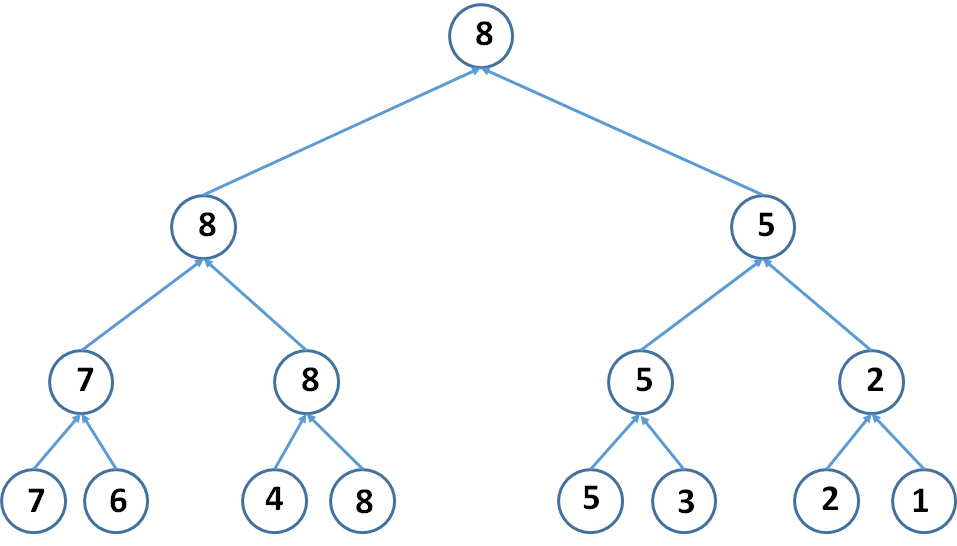
\includegraphics[scale=0.3]{recursiveMaximum.png}
\end{center}

{\bf Analysis:}
\pause
\begin{itemize}
    \item Recurrence Relation: $T(n) = 2T(\frac{n}{2}) + 1 = O(n)$
    \item Number of Comparisons: $n-1$ (Intuition)
\end{itemize}
\end{frame}


\begin{frame}[fragile]{Simultaneous Maximum and Minimum}

{\bf Aim:} Find the maximum and minimum of array $A$ 
\pause
\begin{verbatim}
Minimum-Maximum(A):
    min = Minimum(A)
    max = Maximum(A)
    return min, max
\end{verbatim}
{\bf Analysis:}
\pause
\begin{itemize}
    \item Number of Comparisons: $(n-1)$ + $(n-1)$ = $2n-2$
    \pause
    \item Slightly better: $(n-1)$ + $(n-2)$ = $2n-3$ (for e.g., by swapping min with first element of array)
\end{itemize}
\end{frame}


\begin{frame}{Simultaneous Maximum and Minimum - Visualization}
\begin{center}
    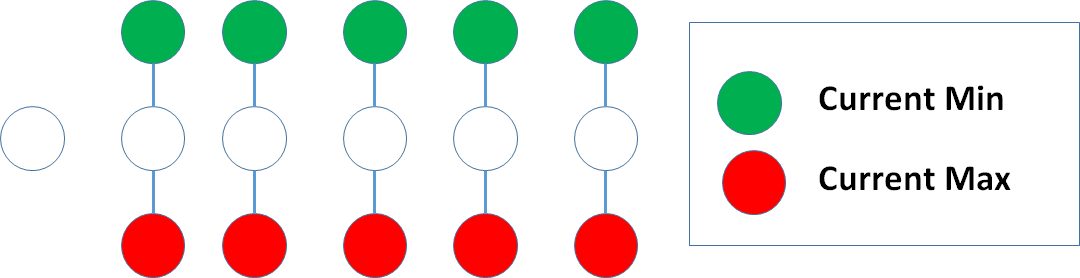
\includegraphics[scale=0.4]{simMinMaxEg1.png}
\end{center}
\end{frame}


\begin{frame}{Simultaneous Maximum and Minimum - Better Algorithm}
\begin{center}
    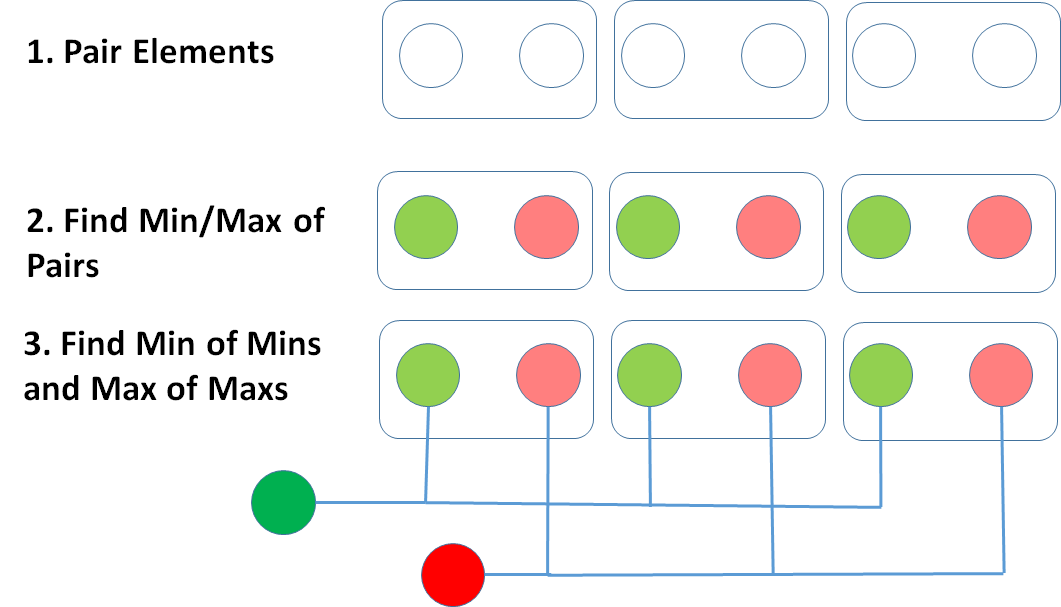
\includegraphics[scale=0.4]{simMinMaxEg2.png}
\end{center}
\end{frame}





\begin{frame}{Simultaneous Maximum and Minimum}

{\bf Analysis:}
\pause
\begin{itemize}
\item Number of Comparisons (approximate): Pairwise + Min of Mins + Max of Maxs
$$(\frac{n}{2}) + (\frac{n}{2}) + (\frac{n}{2})  = \frac{3n}{2}$$
\end{itemize}
\end{frame}




\begin{frame}[fragile]{Finding Second Largest Element - Naive Method}
\pause
\begin{verbatim}
Find-Second-Largest(A):
    max = Maximum(A)
    Swap A[n] with max 
    secondMax = Maximum(A[1:n-1])
    return secondMax
\end{verbatim}
{\bf Analysis:} 
\pause 
\begin{itemize}
\item $n-1$: for finding maximum 
\item $n-2$: for finding 2nd maximum 
\item $2n-3$: total
\end{itemize}

\end{frame}


\begin{frame}[fragile]{Finding Second Largest Element - Tournament Method}
\pause
{\bf Observation:} 
\begin{itemize}
\item In a tournament, second best person could have only be defeated by the best person. 
\item It is not necessarily the other element in the final ``match''
\end{itemize}

\begin{verbatim}
Find-Second-Largest(A):
    max = Recursive-Maximum(A)
    candidates = list of all elements of A that were 
                    directly compared with max
    secondMax = Maximum(candidates)
    return secondMax
\end{verbatim}
\end{frame}


\begin{frame}[fragile]{Finding Second Largest Element - Tournament Method}
\begin{center}
    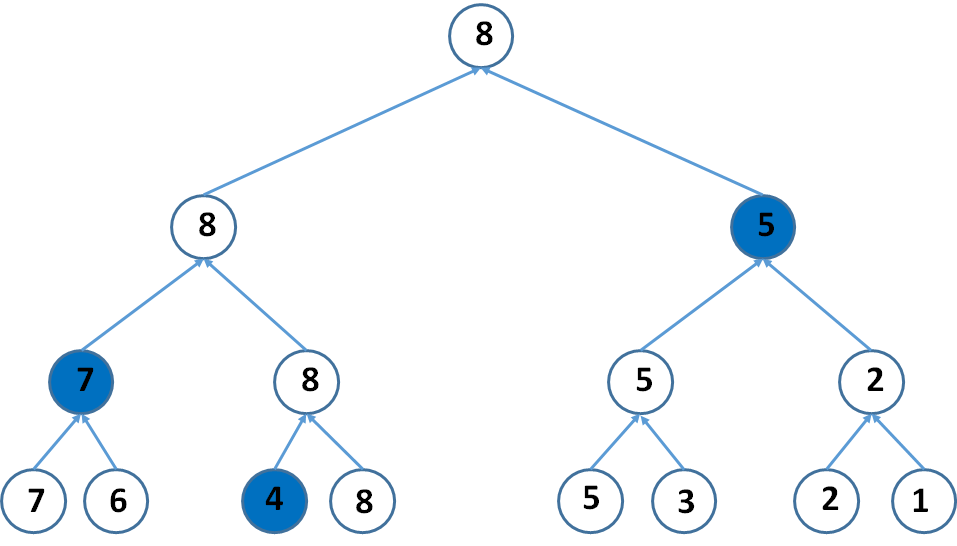
\includegraphics[scale=0.4]{tournamentMethod.png}
\end{center}

{\bf Analysis:} \\
\pause
Number of Comparisons: $ (n-1) + ( \lceil \lg n \rceil - 1) = n +  \lceil \lg n \rceil - 2$
\end{frame}



\begin{frame}{Selection Problem}
\begin{itemize}
\item {\bf Input:} A set $A$ of $n$ (distinct) numbers and an integer $i$ with $1 \leq i \leq n$
\item {\bf Output:} $i^{th}$ smallest element in $A$ 
\item Naive Solution?
\begin{itemize}
    \item Sort $A$ and pick $A[i]$
    \item Time Complexity: $O(n \log n)$
\end{itemize}
\item {\bf Surprising Result}: Can be solved in $O(n)$ time!
\end{itemize}
\end{frame}


\begin{frame}{QuickSelect}
\begin{center}
    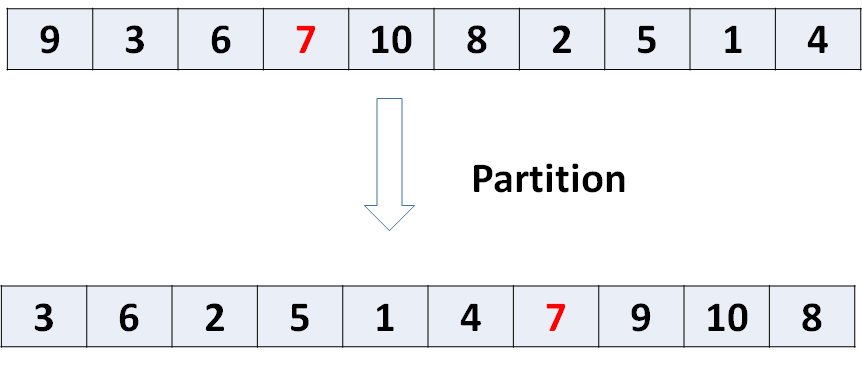
\includegraphics[scale=0.4]{quickSelectCase1.png}
\end{center}
\end{frame}



\begin{frame}{QuickSelect}
\begin{center}
    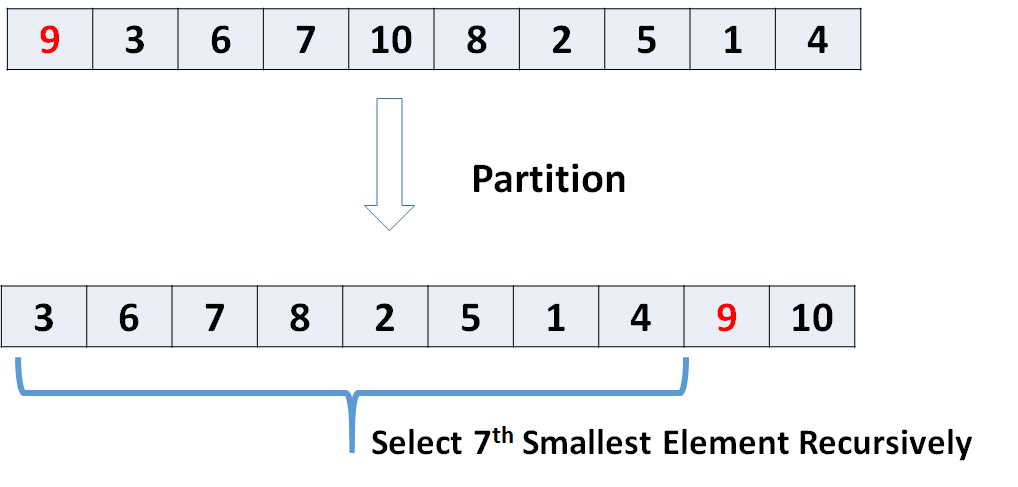
\includegraphics[scale=0.4]{quickSelectCase2.png}
\end{center}
\end{frame}



\begin{frame}{QuickSelect}
\begin{center}
    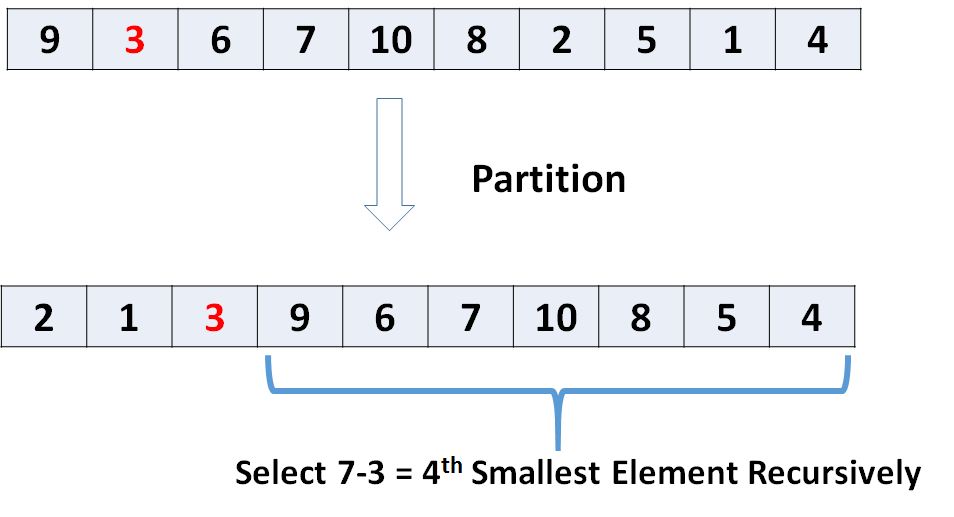
\includegraphics[scale=0.4]{quickSelectCase3.png}
\end{center}
\end{frame}


\begin{frame}[fragile]{QuickSelect PseudoCode}
\begin{verbatim}
Randomized-Select(A, p, r, i)
    if p == r:
        return A[p]
    q = Randomized-Partition(A, p, r)
    k = q - p + 1
    if i == k
        return A[q]
    elseif i < k
        return Randomized-Select(A, p, q-1, i)
    else
        return Randomized-Select(A, q+1, r, i-k)
\end{verbatim}
\end{frame}


\begin{frame}{Radix Sort - LSD Idea}
\begin{center}
%    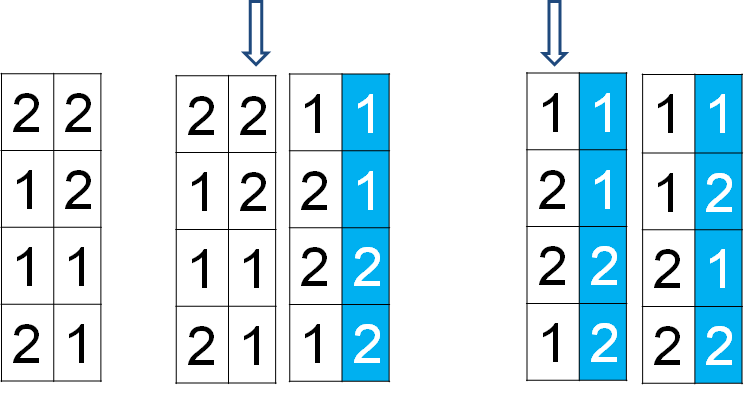
\includegraphics[scale=0.4]{lsdRadixSortEg.png}
GiG
\end{center}
\end{frame}


\begin{frame}{Summary}

\tblue{Major Concepts:}
\begin{itemize}
\item Concept of Lower bounds
\item Lower bounds for Comparison based Sorting Algorithms
\item Decision tree model for Complexity Analysis
\item Linear Time Sorting Algorithms
\end{itemize}
\end{frame}


\end{document}

